\label{section_markers}

To enable the framework to detect a 3D pose from a video feed, a marker with specific properties will be required.
A marker is a visually significant pattern that the system can detect within an image and can be used to calculate spatial coordinates.
Figure \ref{fig:marker_example} shows an example of such a marker.

\begin{figure}
	\centering
	
\includegraphics[width=4cm]{img/marker_example.png}
	\caption[Example Marker.]{An example of a marker. This image is either printed or displayed by some other means in the real world to allow a system to use it as a reference to base a virtual overlay off of it.}
	\label{fig:marker_example}
\end{figure}

Due to our approach for marker detection, we selected a square black on white marker.
Other types exist, such as rotary markers or image-based feature markers.

\section{Coding Scheme}

For this framework, a marker is coded as seen in \ref{fig:marker_template}.
The basis is a six by six sized grid, where the border is solid black.
The internal four by four spaces are used to encode the orientation and identification of the marker.
The orientation is encoded by coloring the corners white except for the top right corner, which is encoded black.
The identification is binary encoded with a Hamming code\cite{hamming} for error detection and correction.
Parity bits are the red bits.

\begin{figure}
	\centering
	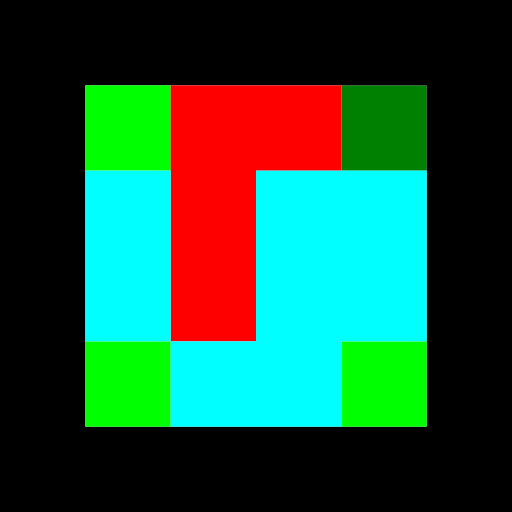
\includegraphics[width=4cm]{img/marker_template.png}
	\caption[Template Marker.]{A color coded representation of a legitimate marker. A real marker is monochrome, the colors here show the location of interesting bits. Green denotes the bits used to determine the rotation: the dark green bit is black, the rest white. Light blue denotes the binary encoded identification number of the marker. Red represents the Hamming encoded parity bits used for error correction.}
	\label{fig:marker_template}
\end{figure}

Thus encoded, the framework can by default detect 256 different markers.
This was deemed sufficient, considering the penalty in performance for each additional detected marker when running on a mobile device, as Imagine becomes unusably slow long before reaching this limit – as seen in section \ref{performance}.

\section{Usage}

Concerning the placement and creation of the marker a few points should be considered.
First off, the framework offers a helper method for creating a binary representation of a marker given an identification number.
This removes any need for the user to manually create and encode a marker and the resulting marker is guaranteed to be correct.

Secondly, the marker should be black on white, with the black border contrasted by white space around it.
Correct detection of the presence of a marker can not be guaranteed otherwise.
Generally speaking, the framework is sensitive to the contrast range of the recorded camera feed, and thus it should be maximized.
Apart from monochrome markers, this also means that the environment should be brightly and constantly lit.

Thirdly, the marker should be created and printed digitally.
The correct detection of the border is the first and most important step in the detection of the marker and should thus be as good as can be managed.
Drawing the markers by hand is possible, but will result in a loss of accuracy due to imperfections that are bound to arise with hand-drawn markers.
Care should especially be taken concerning the outermost border of the marker, as it is the main aspect used for calculating its pose.
This is only true for the border, however: the internal four by four grid containing the orientation and identification of the marker can be drawn in, so long as the drawing is done carefully.

Markers that are not smooth or have other imperfections will either outright fail in being identified or have an incorrect pose assigned to them.
